%%%%%%%%%%%%%%%%%%%%%%%%%%%%%%%%%%%%%%%%%%%%%%%%%%%%%%%%%%%%%
% ECE 445 final paper LaTeX template
% Written by Zhangxiaowen (Andy) Gong
% Created: 03/07/2012
% Last modified: 03/13/2012
%%%%%%%%%%%%%%%%%%%%%%%%%%%%%%%%%%%%%%%%%%%%%%%%%%%%%%%%%%%%%
\documentclass[openbib,letterpaper,10pt]{article}

%%%%%%%%%%%%%%%%%%%%%%%%%%%%%%%%%%%%%%%%%%%%%%%%%%%%%%%%%%%%%
% The preamble starts here.
% You can add other packages that you want to use by using
% \usepackage command in the preamble.
% However, DO NOT change the settings that are already placed
% below unless you really know what you are doing.
%%%%%%%%%%%%%%%%%%%%%%%%%%%%%%%%%%%%%%%%%%%%%%%%%%%%%%%%%%%%%

% some commonly used packages
\usepackage{graphicx}
\usepackage{amsmath}
\usepackage{amsthm}
\usepackage{amsfonts}
\usepackage{setspace}
\usepackage{longtable}
\usepackage{url}
\usepackage{float}
\usepackage{caption}
\usepackage[colorlinks=true,linkcolor=black,citecolor=black]{hyperref}
\usepackage[top=1in, bottom=1in, left=1in, right=1in]{geometry}% set the page margins to 1 inch
\usepackage{siunitx}

% use the fancyhdr package to maintain the format of the page numbers,
% which is useful when the text color is changed
\usepackage{fancyhdr}
\fancyhf{}
\renewcommand{\headrulewidth}{0pt}
\renewcommand{\footrulewidth}{0pt}
\fancyfoot[C]{\textcolor{black}{\thepage}}

% paralist provides extended list environments
\usepackage{paralist}
\setlength{\plitemsep}{0pt}

% define the color for section and subsection titles
\usepackage{xcolor}
\definecolor{titlecolor}{RGB}{31,73,125}
\definecolor{subtitlecolor}{RGB}{79,129,189}

% tikz/pgf environment for making graphs
\usepackage{tikz}
\usepackage{tikz-timing}[2009/12/09]
\usetikzlibrary{shapes,arrows}
\usetikztiminglibrary[new={char=Q,reset char=R}]{counters}

% change the style of the abstract environment
\usepackage{abstract}
\setlength{\absparsep}{6pt}
\setlength{\absleftindent}{0pt}
\setlength{\absrightindent}{0pt}
\setlength{\abstitleskip}{-18pt}
\renewcommand{\absnamepos}{flushleft}
\renewcommand{\abstractnamefont}{\normalfont\Large\singlespacing\bfseries}
\renewcommand{\abstractname}{\textcolor{titlecolor}{Abstract}}

% change the style of the section and subsection titles
\usepackage{titlesec}
\titleformat{\section}{\color{titlecolor}\Large\bf}{\color{titlecolor}\thesection}{0.8em}{}
\titleformat{\subsection}{\color{subtitlecolor}\large\bf}{\color{subtitlecolor}\thesubsection}{1em}{}
\titleformat{\subsubsection}{\color{subtitlecolor}\normalsize\bf}{\color{subtitlecolor}\thesubsubsection}{1.2em}{}
\titlespacing{\section}{0pt}{0em}{0em}
\titlespacing{\subsection}{0pt}{0em}{0em}
\titlespacing{\subsubsection}{0pt}{0em}{0em}

% change the style of the table of contents
\usepackage{titletoc}
\titlecontents{section}[1.5em]{}{\contentslabel{1.5em}}{\hspace*{-1.5em}}{\titlerule*[0.5pc]{.}\contentspage}
\titlecontents{subsection}[3em]{}{\contentslabel{2.1em}}{\hspace*{-2.1em}}{\titlerule*[0.5pc]{.}\contentspage}
\titlecontents{subsubsection}[5.1em]{}{\contentslabel{2.7em}}{\hspace*{-2.7em}}{\titlerule*[0.5pc]{.}\contentspage}

% command for centering texts in a fixed width table cell
\newcommand{\centpcol}{\leftskip\fill \rightskip\fill}

% command for setting the style of the appendix titles
\newcommand{\setappenstyle}{
	\titleformat{\section}{\color{titlecolor}\Large\bf}{\color{titlecolor}Appendix \Alph{section}}{0.8em}{}
	\titlecontents{section}[0em]{}{Appendix \thecontentslabel \hspace{1em}}{}{\titlerule*[0.5pc]{.}\contentspage}
}

% define the style of the title of the paper
\newcommand{\thetitle}[1]{\title{\begin{Huge}{\bf #1}\end{Huge} \color{subtitlecolor}\rule[25pt]{\textwidth}{1pt}}}

% define the style of the author
\newcommand{\theauthor}[3]{
	\author{\vspace{0.5in}\\
	\textcolor{black}{By}\\
	#1
	\vspace{0.8in}\\
	\textcolor{black}{Final Report for ECE 445, Senior Design,} #2\\
	\textcolor{black}{TA:} #3
	\vspace{0.3in}}
}

% define the style of figure's caption
\newcommand{\figcap}[1]{
	\captionsetup{format=plain,font={small,color=subtitlecolor,singlespacing},margin={0pt,0pt}}
	\caption{\textcolor{subtitlecolor}{#1}}
	\vspace{-5pt}
}

% define the style of table's caption
\newcommand{\tablecap}[1]{
	\captionsetup{format=plain,font={bf,normalsize,singlespacing,color=black},margin={0pt,0pt}}
	\caption{\textcolor{black}{#1}}
	\vspace{-5pt}
}

% define the style of the abstract's page number
\newcommand{\abstractsetting}{
	\pagenumbering{roman}
	\thispagestyle{fancy}
}

\newcommand{\buildtoc}{
	\clearpage
	\singlespacing
	\tableofcontents
	\clearpage
	\onehalfspacing
	\setcounter{page}{1}
	\pagenumbering{arabic}
}

% set indentations and the space between paragraghs
\setlength{\parindent}{0pt}
\setlength{\parskip}{8pt}

%%%%%%%%%%%%%%%%%%%%%%%%%%%%%%%%%%%%%%%%%%%%%%%%%%%%%%%%%%%%%
% The preamble ends here.
%%%%%%%%%%%%%%%%%%%%%%%%%%%%%%%%%%%%%%%%%%%%%%%%%%%%%%%%%%%%%

\begin{document}

% don't change these
\pagestyle{empty}
\doublespacing

% put the title of your project here. DO NOT include the brackets.
\thetitle{Beacon-Controlled Autonomous Network for Trains (BCAN’T)}

% put your names here. seperate by \\. DO NOT include the brackets.
\theauthor{
	Susan Chen\\
	Prithvi Garimalla\\
	Jordi Pakey-Rodriguez
}
{ % put the semester info here. DO NOT include the brackets.
	Spring 2017
}
{ % put your TA's name here. DO NOT include the brackets.
	Jacob Bryan
}

% put the date and project number here. DO NOT include the brackets.
\date{
03 May 2017\\
Project No. 5
\clearpage
}

% don't change these
\maketitle
\pagestyle{fancy}
\begin{spacing}{1.15}

% put the abstract here
\begin{abstract}
BCAN’T is a system for model trains that consists of infrared beacons and a laser time-of-flight sensor in order to enable true “set and go” operation. Over the course of the project we developed the beacon reading system and it demonstrated it works, as well as a complete control system on the locomotive that interfaces the beacon and time-of-flight data to control to motor and other peripherals. Unfortunately, due to last minute hardware failures, we were unable to integrate all the components onto a locomotive, but most of the components were demonstrated to work on their own.
\abstractsetting % do not delete this line
\end{abstract}

% build the table of contents.
\buildtoc


\section{Introduction}
\subsection{Objective}
Model trains have become more and more advanced over the last few decades, but they are still controlled entirely by a human operator. These human operators are solely responsible for ensuring that no harm comes to the train. A lapse in attention can be disastrous, causing damage that could be very costly to repair. Model trains currently do not have the ability to detect obstacles or other trains in front of them. If not stopped in time a crash may occur, often resulting in derailment or physical damage. Additionally, derailment may occur when a train is traveling at high speeds on a curved tracks. The train has no recourse for these situations other than for the operator to manually slow or stop it to avoid an accident.\par

Currently, the National Model Railroad Association (NMRA) defines the Digital Command Control (DCC) standard for model trains. DCC allows for digital control of various train functions such as lights, speed, direction, sound, and much more\cite{NMRA_DCC}. One downside to DCC is that smooth operation is completely dependent on the human operator who must manually control the train as it is unable to react to its environment autonomously. In addition, DCC has a steep learning curve and setting up a system without prior experience can be quite challenging.\par

Our solution is to give each locomotive the ability to respond to the track on its own by detecting obstacles and reacting to programmable beacons placed on the track. A distance sensor is placed on the front of the train to detect obstacles directly in front of it. Small beacon modules placed on the track are set to send out unique identifiers to the train to let it know what speed it should travel at. Essentially, the end goal is to have the train sense potential issues along the track that would cause collision or derailment and act to avert such problems. Our solution is a convenient alternative to those who wish to have speed control for their locomotives. The sensors integrated with the locomotive also provide some measure of protection against human negligence by avoiding obstacles and preventing derailment.

\subsection{High-Level Requirements}
\begin{itemize}
\item Must be able to operate indefinitely on existing methods of track power, both analog (DC) and bipolar Digital Command Control (DCC).
\item Must be able to detect oncoming obstacles on the track and stop to avoid derailment or damage.
\item Must be able to read customizable speed limit beacons that are powered by the tracks and adjust its speed accordingly.
\end{itemize}

\clearpage

\section{Design}
Our solution consists of two independent systems: the beacon boards and the locomotive controller. The beacons are small standalone boards on the track that continuously broadcast a unique ID that is read as the train passes over. The locomotive controller consists of three PCB’s on the train and is responsible for reading beacons, identifying obstacles, and controlling the motor. The block diagram is shown in Figure 1.

\begin{figure}[H]
\begin{center}
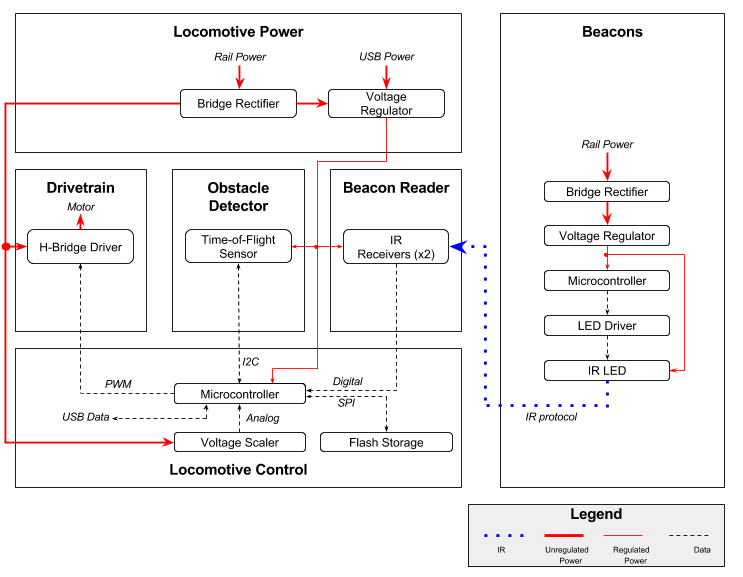
\includegraphics[height=36em]{img/block_diagram.png}
\figcap{Block Diagram.}
\end{center}
\end{figure}

\subsection{Beacon}
The beacon is small board that sits between two track ties as shown in Figure 2. The image on the left shows the placement of a beacon on the track, and the image on the right shows three individual beacons with their ID labels. Its function is to broadcast a unique ID to the IR receiver board on the locomotive. Each ID is mapped to a specific function that can be programmed on the locomotive control board. A bridge rectifier and a voltage regulator are used to provide 2.8V power to the microcontroller, LED driver, and IR LED. The microcontroller controls the IR LED to continuously broadcast the board’s ID for the IR receiver on the locomotive board to read.

\begin{figure}[H]
\begin{center}
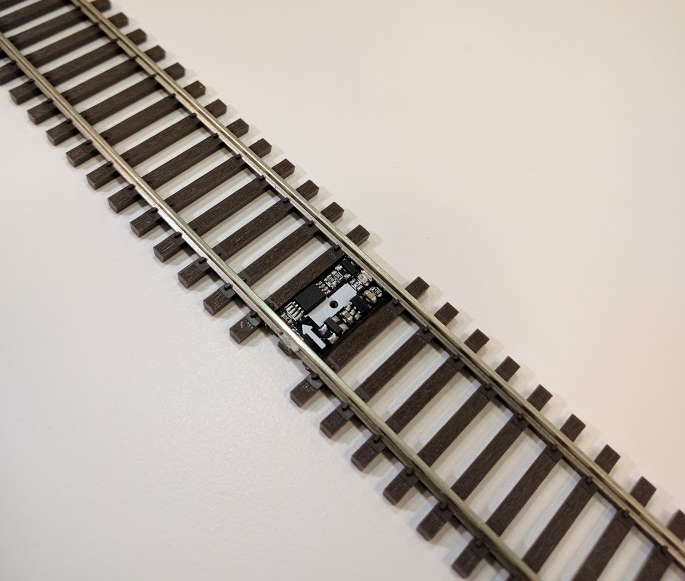
\includegraphics[trim={80 70 90 80},clip,height=18em]{img/beacon_track.png}
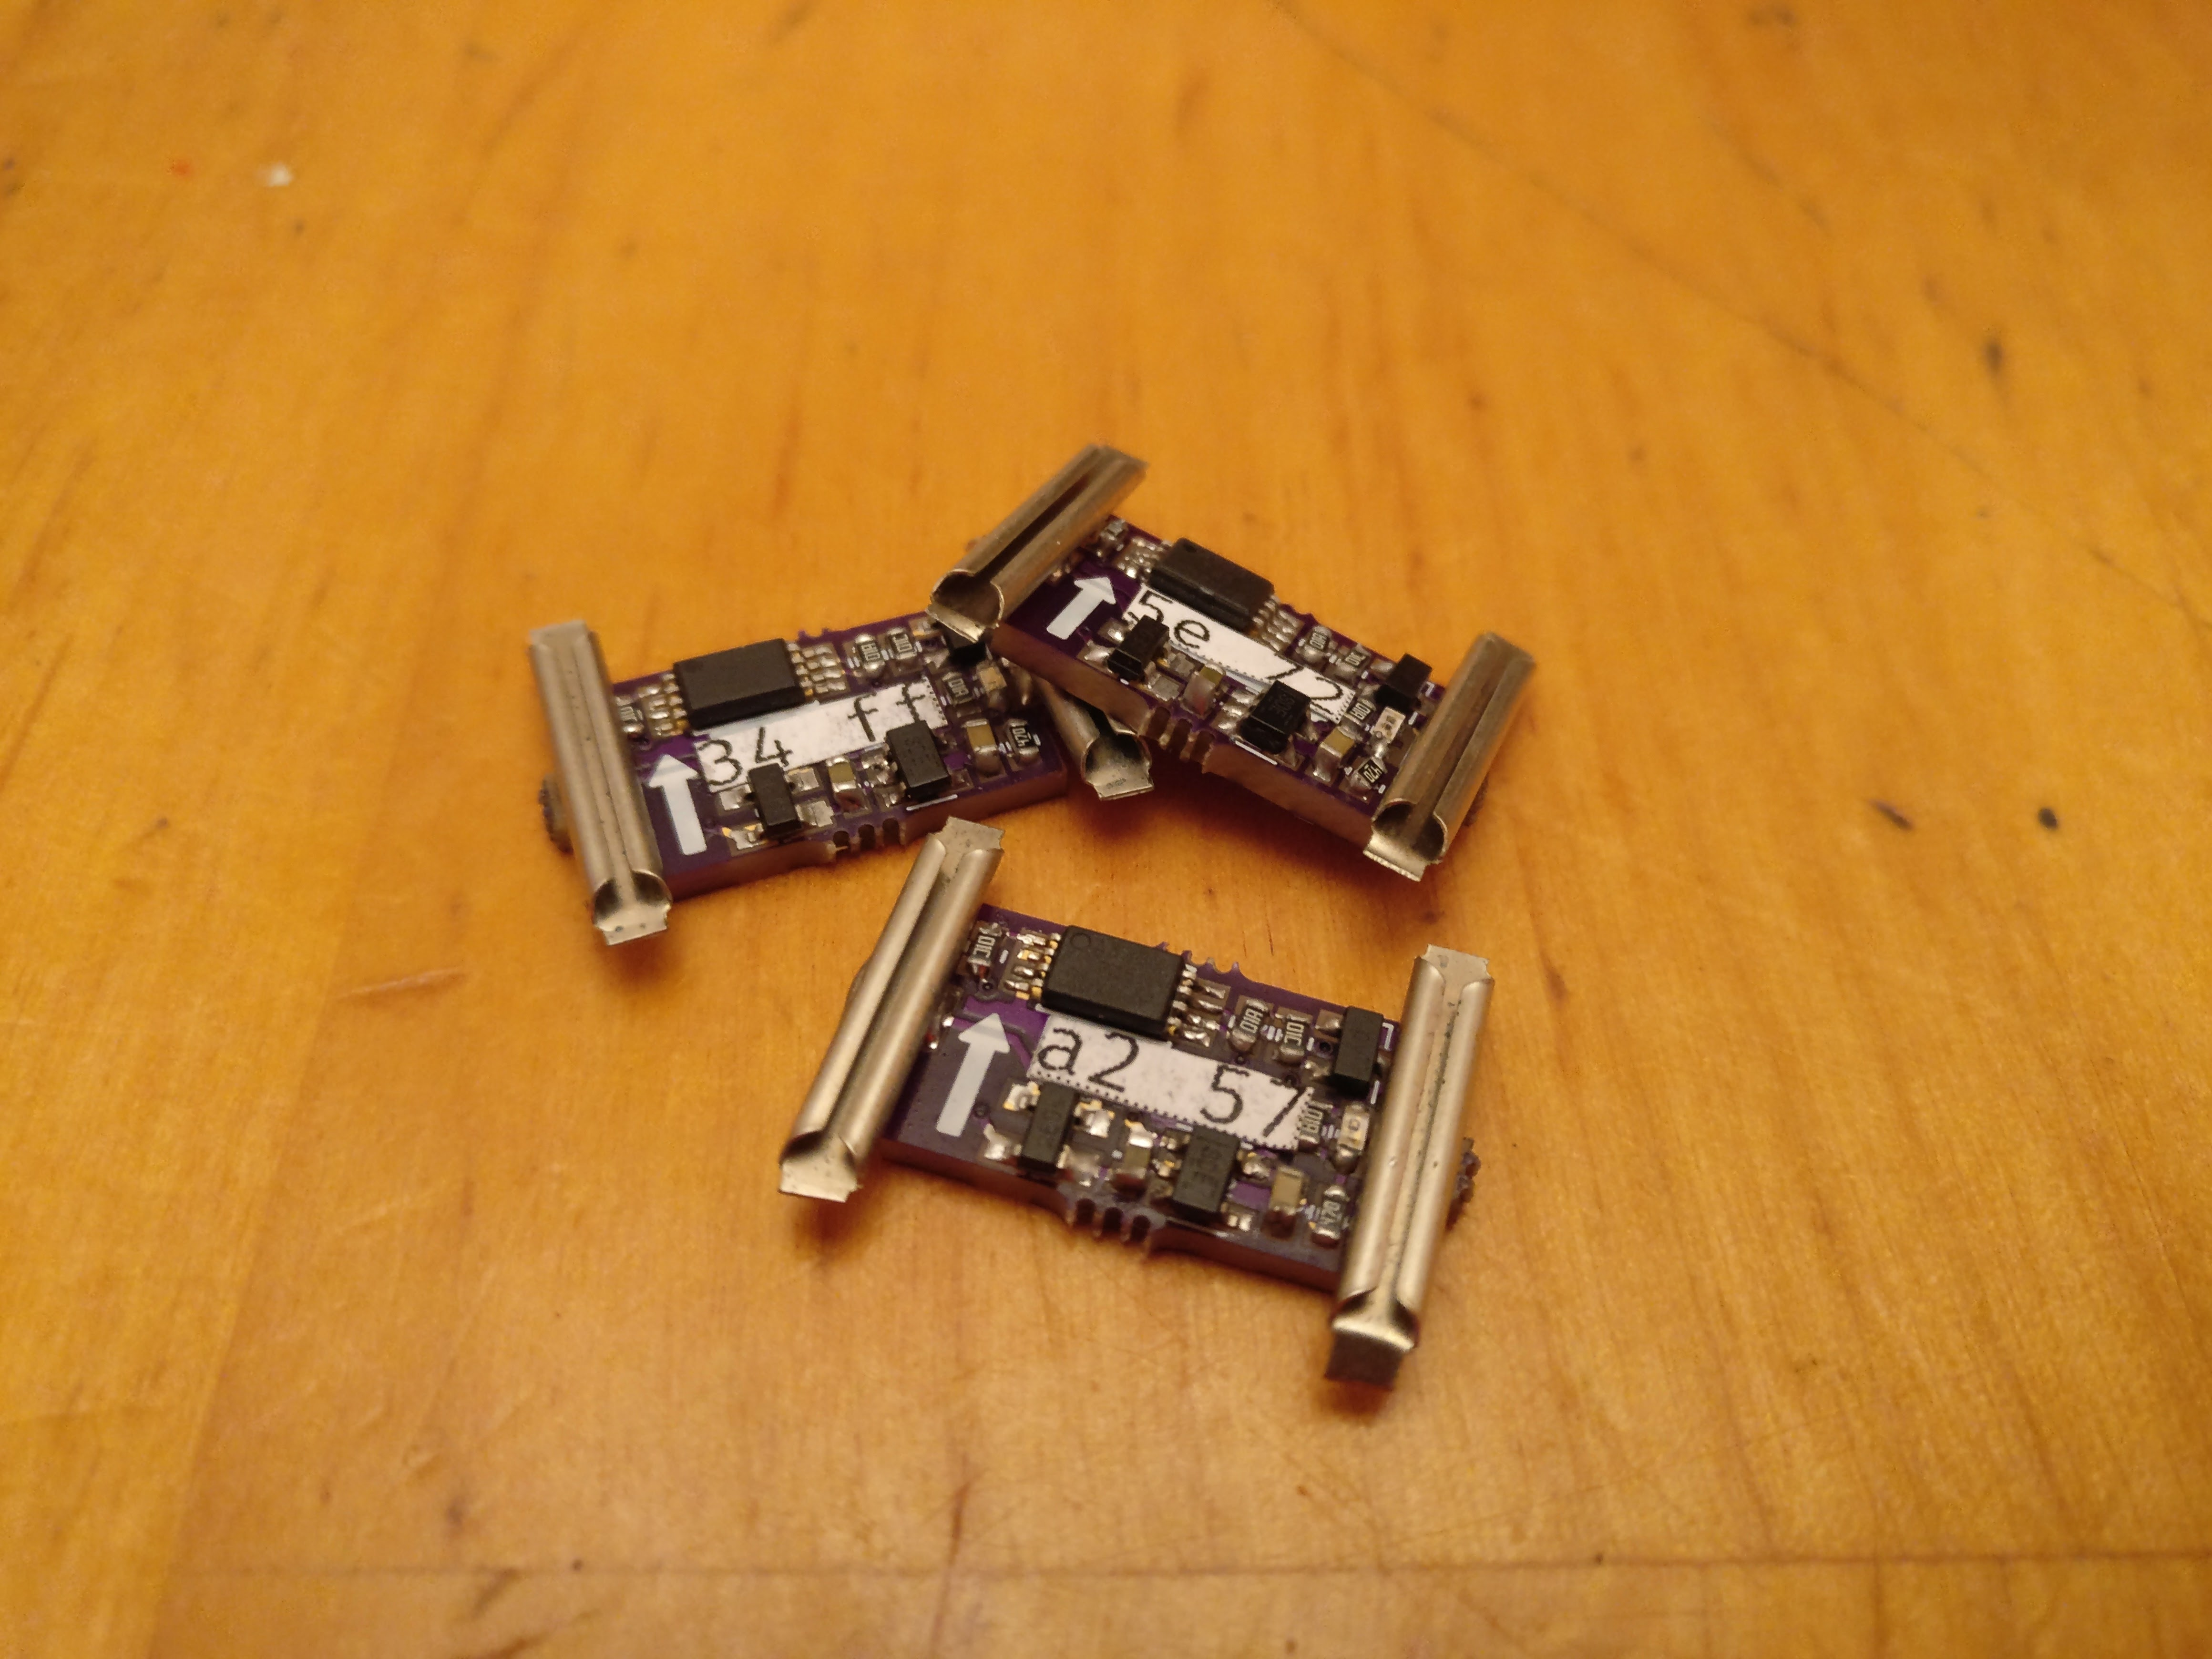
\includegraphics[trim={800 400 800 600},clip,height=18em]{img/beacon_boards.jpg}
\figcap{Beacon Boards.}
\end{center}
\end{figure}

\subsubsection{Schematic}
The schematics for the beacon board IR LED and power circuits are shown in Figure 3 and Figure 4, respectively. The shunt resistor R5 is used to create a clean 38kHz modulated signal since the LED is unable to switch fast enough. The calculations for R2 and R4 are shown in Calculations 1 and 2 in Appendix B.

\begin{figure}[H]
\begin{center}
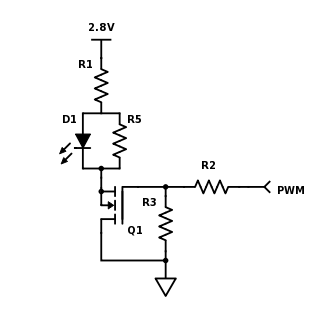
\includegraphics[height=15em]{img/beacon_led.png}
\figcap{Beacon IR LED Circuit.}
\end{center}
\end{figure}

\begin{figure}[H]
\begin{center}
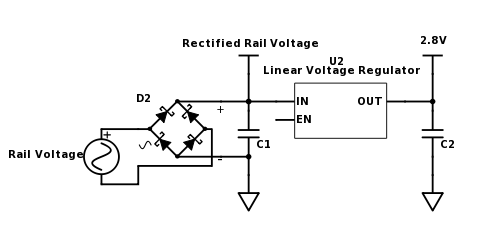
\includegraphics[height=12em]{img/beacon_power.png}
\figcap{Beacon Power Circuit.}
\end{center}
\end{figure}

\subsubsection{Bridge Rectifier}
Since the voltage regulator only takes positive voltage, the full-bridge rectifier is needed rectify the power signals from the rails. It consists of four schottky diodes in a bridge configuration and rectify rail voltages ranging from -16V to +16V.

\subsubsection{Voltage Regulator}
A linear voltage regulator takes an input from the rectified rail power and bring the voltage down to 2.8V from an input voltage of up to 16V. It provides the power needed for the MCU and its peripherals.\par

The TPS709 linear voltage regulator data sheet specifies a minimum input voltage of 2.7V\cite{TPS709}. Testing showed that an input voltage of 3.5V would produce an output voltage of 2.63V, while input voltages lower than 3.5V would produce an output voltage that is below our requirements. Therefore, a input voltage of 3.5V would be the minimum threshold for our project to function properly.

\subsubsection{Microcontroller}
The microcontroller used is an ATtiny45 8-bit AVR processor. It uses a single GPIO pin to control the LED driver circuit and continuously broadcast the board’s unique ID using the IR protocol.

\subsubsection{LED Driver}
The LED driver circuit consists of an N-channel MOSFET, a gate resistor, and a pull down resistor. The MOSFET conducts current when the I/O pin from the microcontroller is set to high. The gate resistor is used to prevent damage due to overcurrent to the microcontroller and the pull down resistor is used to ensure the MOSFET is turned off when the voltage at the gate is left floating.

\subsubsection{IR LED}
The 940nm IR LED is used to broadcast a unique ID that the receiver on the locomotive can read. It is controlled by the LED driver circuit using PWM. The viewing half-angle for the LED can be calculated using Equation 1. The calculation for the viewing half angle can is shown in Calculation 3 in Appendix B.

\begin{equation}
\theta_{\frac{1}{2}}=\arctan\bigg(\frac{V_{max}T}{2H_{min}}\bigg)
\end{equation}

Vmax is the max speed of the train, T is the length of one ID message, and Hmin is the minimum distance from the beacon board LED to the IR receivers on the train.

\subsection{Locomotive Power}
The locomotive power circuit takes an input voltage ranging from -16V to +16V from the rail or 5V from the USB. It then rectifies and regulates that voltage down to 2.8V in order to power the microcontroller and its peripherals. A full bridge rectifier is used to rectify the AC voltage from the rails. The rectified voltage is then inputted to a linear voltage regulator. The SPX3918 adjustable linear voltage regulator has a minimum input voltage of 2.5V and a maximum dropout voltage of 550mV with a 500mA current draw. This means the minimum input threshold voltage in order for the locomotive components to be powered would be 3.35V, allowing for the microcontroller to be able to wait for the input voltage to reach the 3.5V minimum threshold limit for the beacon board to be powered. The circuit for the locomotive power block is shown in Figure 5.\par

Other designs were considered for the locomotive power circuit. A switching circuit to switch between the USB power source and the rail power source was considered. However, it was simpler to add a protection diode after the USB voltage source. There were also attempts to regulate the input voltage through the full range of rail voltages with switching circuits, switch-mode power supplies, or batteries. The switching circuits were complex and risked shorting the input and output voltages if the timing was not correct. There were no switch-mode power supplies on the market that had a low enough input voltage for the output that was required. Batteries would have defeated the purpose of drawing power from a wall outlet.

\subsubsection{Schematic}
\begin{figure}[H]
\begin{center}
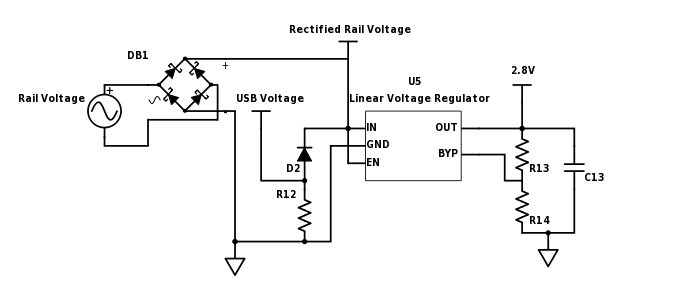
\includegraphics[height=15em]{img/locomotive_power.png}
\figcap{Locomotive Power Schematic.}
\end{center}
\end{figure}

\subsubsection{Bridge Rectifier}
The full-bridge rectifier is needed to rectify power signals from the rails before they are routed to the voltage regulator, voltage scaler, and motor driver. It consists of four schottky diodes in a bridge configuration and rectifies voltages ranging from -16V to +16V.

\subsubsection{Voltage Regulator}
The rectified voltage is fed into a linear voltage regulator in order to bring the voltage down to 2.8V. The 2.8V source is used to power the microcontroller, time-of-flight sensor, IR receiver, and the voltage scale circuit. Calculation 4 in appendix B shows how the adjustment resistors are calculated for the SPX3819 linear regulator for an output voltage of 2.8V using Equation 2.

\begin{equation}
V_{out}=1.235(1+\frac{R_1}{R_2})
\end{equation}

\subsection{Locomotive Control}
The locomotive control unit consists of a microcontroller and a USB data connection. If there is a USB connection the control unit will enter a programming mode, otherwise it will run the normal track operation. This allows operators to map the beacon IDs to one of 128 different speeds\cite{NMRA_Standard}. The microcontroller receives a voltage input via the ADC pin from the voltage scale circuit and outputs a PWM signal to the drivetrain to control the speed. The IR receiver sends beacon IDs to the microcontroller in order to determine what speed the train should go. It also stops the train if the time-of-flight sensor detects an obstacle in its path.

\subsubsection{Schematic}
The main part of the control circuit is the STM32F4 microcontroller. It is connected to a M95512-RDW6TP EEPROM for storage of the beacon mappings. The control schematic is shown in Figure 6.

\begin{figure}[H]
\begin{center}
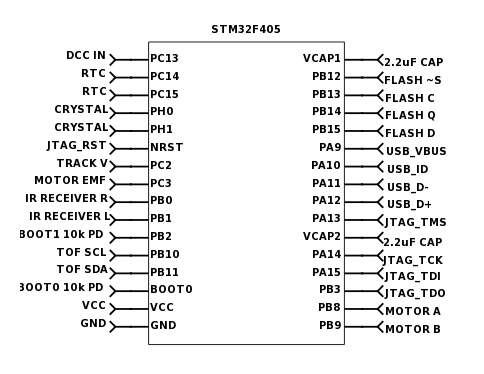
\includegraphics[height=18em]{img/locomotive_control.png}
\figcap{Locomotive Control Schematic.}
\end{center}
\end{figure}

\subsubsection{Microcontroller}
The microcontroller used is an STM32F405 32-bit ARM processor. It communicates with the time-of-flight sensor via I2C, the IR receiver digitally, and control the motor with PWM signals. It also stores configuration data for the beacons in external memory.

\subsubsection{Flash Storage}
An EEPROM flash chip is used to store the beacon mappings. It communicates with the microcontroller over SPI. EEPROM was chosen since we can address individual bytes, which makes performing binary search through the dataset for the beacon mappings more efficient.

\subsubsection{Voltage Scaler}
The voltage scaler circuit originally included an operational amplifier buffer to improve the accuracy of the voltage readings. However, we were unable to find an operation amplifier that could be powered by a 2.8V source, so errors were corrected in software instead. The voltage scaler circuit consists of a resistive voltage divider, shown in Figure 7, that scales the rectified rail voltage down to a lower voltage that can be read by the microcontroller’s ADC. The rectified rail voltage ranges from 0-16V and the microcontroller ADC can read voltages from 0-2.8V. Two resistors divide the voltage to output a range of 0-2.8V, which will give 4096 different values for a 12-bit precision ADC. The calculations using Equation 3 of the voltage divider's resistor values are shown in Calculation 5 in appendix B.

\begin{figure}[H]
\begin{center}
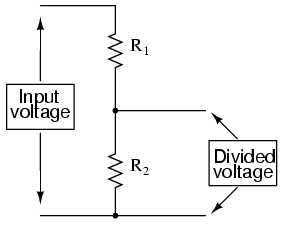
\includegraphics[height=12em]{img/voltage_divider.png}
\figcap{Voltage Divider Circuit.}
\end{center}
\end{figure}

\begin{equation}
V_{out}=V_{in}\frac{R_2}{R_1+R_2}
\end{equation}

\subsection{Locomotive Drivetrain}
The locomotive drivetrain unit consists of the motor controller circuit that interfaces the PWM signal from the microcontroller with the rectified rail power in order to power the motor. The circuit consists of a MOSFET H-bridge that is gate-driven by NPN transistors. The drivetrain circuit is shown in Figure 8.\par

In order to drive the MOSFETs in the H-bridge, optoisolators were also considered. However, we were unable to find an optoisolator that would support driving the LED with our maximum rectified rail voltage.

\subsubsection{Schematic}
\begin{figure}[H]
\begin{center}
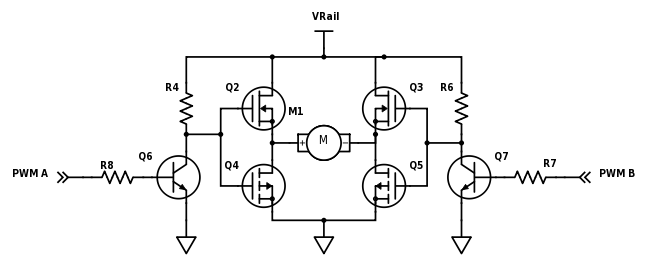
\includegraphics[height=15em]{img/locomotive_drivetrain.png}
\figcap{Locomotive Drivetrain Schematic.}
\end{center}
\end{figure}

\subsubsection{Motor Controller}
The motor driver circuit consists of two PWM signals driving two NPN transistors which each control an NFET and a PFET. The MOSFETs are configured as an H-bridge and allow the motor to run forwards or backwards at any speed determined by the PWM signals. The frequency of the PWM signals is 10kHz to prevent resonance and noise. The motor current range is $\pm$1.5A and the motor voltage range is $\pm$16V.

\subsection{Obstacle Detector}
The obstacle detector consists of a time of flight (TOF) sensor mounted to the front of the train. It detects any obstruction on the tracks that could cause the train to derail and cause an emergency stop. The TOF sensor uses a laser to measure whether the path in front of the train is clear or if the train is approaching an unexpected obstacle. The range of the TOF sensor is approximately 50-200mm\cite{VL6180X}.

\subsection{Beacon Reader}
The beacon reader consists of two IR receivers mounted underneath the train on either side. They read beacons as the train passes over them. With two receivers, the microcontroller can infer the direction the train is moving and execute different actions accordingly.

\subsection{IR Protocol}
The IR protocol uses 38kHz modulation present in many televisions and other consumer devices. We chose this frequency because sensors for it are widely available. Our protocol uses Manchester encoding according to the G.E. Thomas convention with a bit period of 960s and data length of 16 bits\cite{Manchester}. The timing diagram for the protocol is shown in Figure 9.

\begin{figure}[H]
\begin{center}
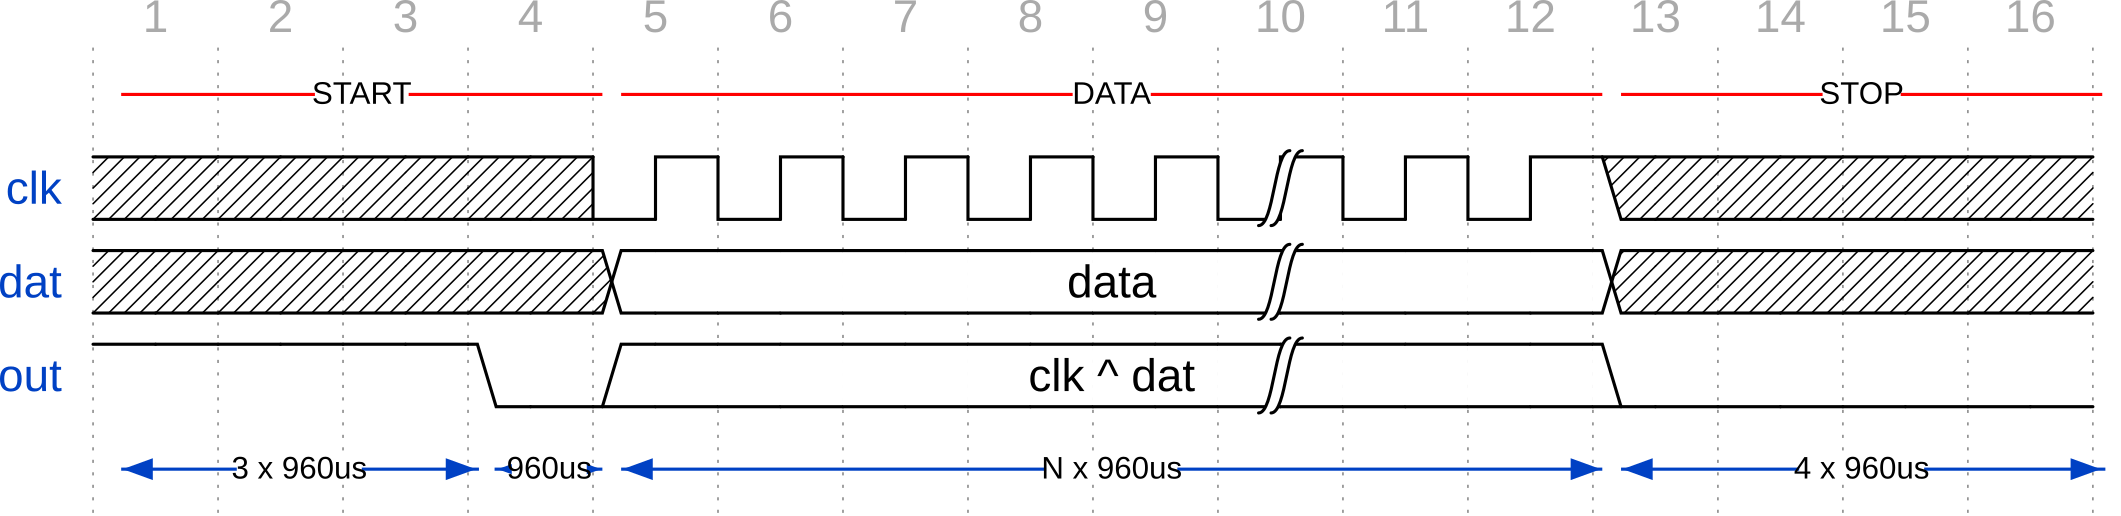
\includegraphics[height=9em]{img/ir_protocol.png}
\figcap{IR Protocol Timing Diagram.}
\end{center}
\end{figure}

\subsection{Beacon Firmware}
The beacon firmware is a simple loop that continuously broadcasts the beacon ID using the IR protocol. Every 480us it determines what the next edge is (rising or falling) and sets the GPIO pin accordingly.

\subsection{Locomotive Firmware}
The locomotive has two modes of operation: track mode and programming mode. It also reacts to pin change interrupts from the IR receiver. At boot, the microcontroller checks to see if USB is connected. If so, it enters programming mode and presents itself as a USB mass storage device. When the user starts to write a configuration file to the locomotive, the microcontroller will buffer each beacon mapping and verify they are being written in ascending order. This is required since at look-up time, it will perform a binary search through the mappings to find the correct one. If an errored mapping comes in, the microcontroller will stop storing more mappings.\par

In track mode, the microcontroller will continuously check the obstacle detector, stopping the train if there is one. Then it checks whether a beacon ID is read and looks up the appropriate mapping before executing it. Finally, it makes any motor adjustments as necessary.\par

The IR receiver also works by invoking a pin change interrupt every time its value changes. Using our IR protocol and taking advantage the repetitive pattern of the data we are sending, we need only store one message length worth of pin changes to calculate the beacon ID. When we have the requisite data, we set a “ready flag” which will trigger the main event loop to look up and execute the mapping.

\subsubsection{Feature List}
\begin{itemize}
	\item Mount as USB mass storage device if USB plugged on boot
	\item Stores the beacon mappings on flash memory
	\item Reads beacons through pin change interrupts
	\item Can stop the train if an obstacle is detected
	\item Can continuously adjust the motor speed and direction based on track conditions
\end{itemize}

\subsubsection{Flow Chart}
The flowchart for the locomotive operation is is shown in Figure 10.

\begin{figure}[H]
	\begin{center}
		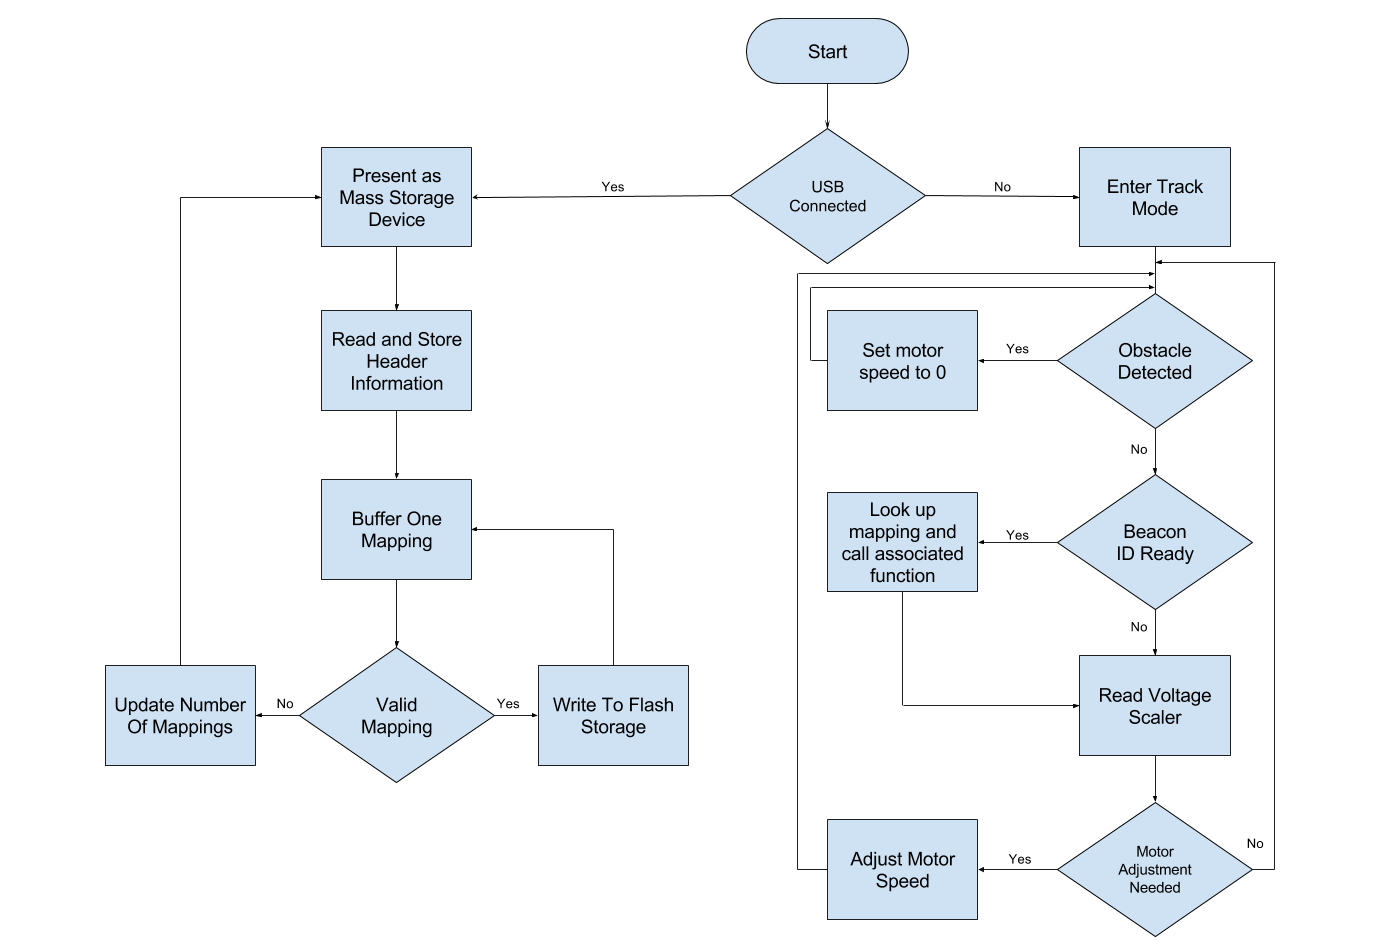
\includegraphics[height=32em]{img/locomotive_flowchart.png}
		\figcap{Locomotive Firmware Control Flow.}
	\end{center}
\end{figure}

\subsection{PC Software}

\subsubsection{Beacon Configurator}
Figure 11 shows the web interface (hosted online \href{http://jordi.codes/bcan}{here}
) to program the beacons. Once specifying the ID, the user can select the instances where the mapping applies and the action the beacon corresponds to.

\begin{figure}[H]
	\begin{center}
		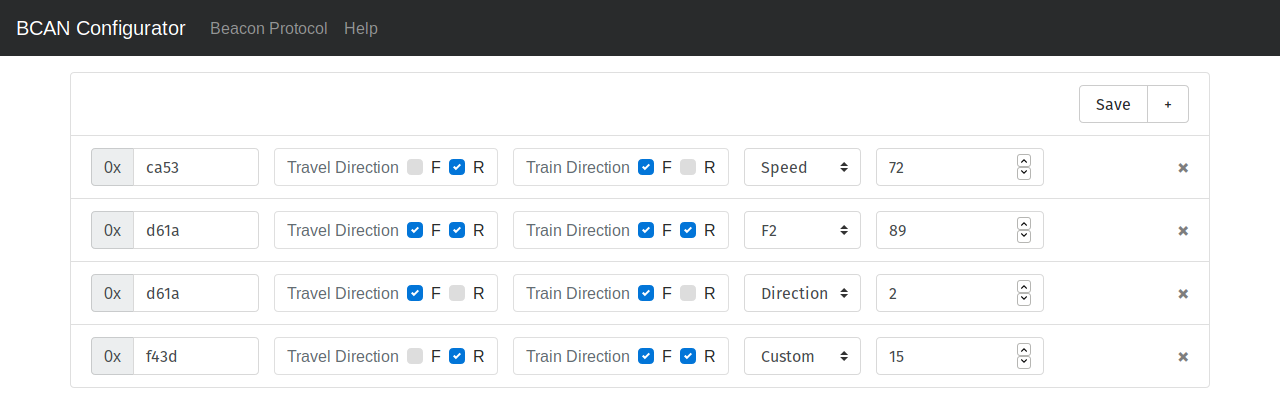
\includegraphics[height=15em]{img/beacon_configurator.png}
		\figcap{Beacon Configurator Website.}
	\end{center}
\end{figure}

\subsubsection{Feature List}
\begin{itemize}
	\item Allows user to add any number of beacon mappings
	\item Each mapping consists of a beacon ID, description, direction of travel, direction of drain, function, and additional parameters for that function
	\item Clicking “Save” downloads a file that can be copied to the USB mass storage device to program the mappings
\end{itemize}

\clearpage

\section{Cost}
In order to keep costs low, we chose a locomotive microcontroller that can be switched out with a cheaper one in case the user did not require as many peripherals. We also kept the locomotive board limited to 2 layers as a 4 layer board would have significantly increased the price. On the beacon side, we kept the BOM to under \$5 in single quantities, and have already designed a v2.0 with a cheaper microcontroller that has a \$1 BOM at quantity 1000.

\subsection{Labor}
\begin{center}
\begin{longtable}{|c|c|r|r|r|}
\tablecap{Labor Costs}
		\\
		\hline \multicolumn{1}{|p{10em}|}{\centpcol\textbf{Name}} & \multicolumn{1}{p{10em}|}{\centpcol\textbf{Total Hours}} & \multicolumn{1}{p{7em}|}{\centpcol\textbf{Hourly Rate (\$)}} & \multicolumn{1}{p{7em}|}{\centpcol\textbf{Total (\$)}} & \multicolumn{1}{p{7em}|}{\centpcol\textbf{Total * 2.5 (\$)}}\\ \hline
		\endfirsthead

		\multicolumn{5}{c}
		{{\bfseries \tablename\ \thetable{} -- continued from previous page}} \\
		\hline \multicolumn{1}{|p{10em}|}{\centpcol\textbf{Name}} & \multicolumn{1}{p{10em}|}{\centpcol\textbf{Total Hours}} & \multicolumn{1}{p{7em}|}{\centpcol\textbf{Hourly Rate (\$)}} & \multicolumn{1}{p{7em}|}{\centpcol\textbf{Total (\$)}} & \multicolumn{1}{p{7em}|}{\centpcol\textbf{Total * 2.5 (\$)}}\\ \hline
		\endhead

		\hline \multicolumn{5}{|r|}{{Continued on next page}} \\ \hline
		\endfoot
		\endlastfoot
			Susan Chen & 170 & 36.00 & 6,120.00 & 15,300.00 \\ \hline
			Prithvi Garimalla & 170 & 36.00 & 6,120.00 & 15,300.00 \\ \hline
			Jordi Pakey-Rodriguez & 170 & 36.00 & 6,120.00 & 15,300.00 \\ \hline
			\textbf{Total} & 510 & 108.00 & 18,360.00 & 45,900.00 \\ \hline
	\end{longtable}
\end{center}

\subsection{Parts}
We spent \$200 on parts which, combined with our \$45,900 labor costs, gives a total project cost of \$46,100.

\clearpage

\section{Conclusion}

\subsection{Accomplishments}
While our project definitely had some issues that kept it from being a complete success, the most critical and innovative part, beacon reading, worked. It was demonstrated to be versatile and the speed at which the IDs could be read exceeded our expectations. Furthermore, we designed the project to be as economical as possible, so the total cost of the materials for a beacon was quite cheap. Should there be demand for this product in the model train community, we believe there would be a legitimate path to market.
% \vspace{0.2in}

\subsection{Uncertainties}
We still have a few lingering questions about our project, namely the nature of the eleventh hour failure we experienced. We had soldered the locomotive board and it had been working for two weeks until a short developed two days before the final demo. After thinking we had identified the cause and replaced the suspect component, another short, this time at the output of the 2.8V voltage regulator appeared. This was approximately 18 hours before our final demo and the only solution we saw was to solder together another board. Unfortunately, even though this board had never even been powered, the short was still present. Even after thoroughly examining the board under a microscope, the only theory we have for the second board being faulty is a faulty component. At this point, even though we were able to demonstrate the individual aspects of the project worked, integrating them was not successful.
% \vspace{0.2in}

\subsection{Ethical considerations}
There are two potential safety concerns with our project, however we believe they are both within the acceptable tolerances for a general consumer product. The first of these is that the rails of the train track are electrically charged so one could potentially shock themselves. However, we are not changing this characteristic in our design and therefore are not creating any additional safety hazards. This is a well understood risk of model trains so responsible usage dictates they should be kept out of reach of small children or pets. The second is that we are using a time-of-flight sensor that uses a laser. The laser used is Class 1, which means that it is safe for use under normal conditions and while operating within the manufacturer's specifications\cite{VL6180X}.\par

In accordance with the IEEE code of ethics, we endeavored to take on technical tasks we feel we are qualified for and seek advice from our mentors for the skills we lack. We sought feedback and criticism for our work and continuously worked to correct our mistakes. We strove for honesty and properly credited individual contributions to our project. Most importantly, we supported and encouraged each other to follow this code of ethics.
% \vspace{0.2in}

\subsection{Future work}
The software, firmware, and schematics for our project are fully open source and there is no reason why the work on our project has to stop here. Our design choices and decisions are well documented, so should anyone choose to continue our work, they can easily pick up where we left off. We have already designed a v2.0 beacon, and have made a list of changes for the next locomotive version.
% \vspace{0.2in}

\clearpage

\bibliographystyle{IEEE_ECE}
% include the BibTex file here to build reference
\bibliography{final_report}\addcontentsline{toc}{section}{Reference}

\clearpage
\setappenstyle
\begin{appendix}
\section{Requirement and Verification Tables}

\begin{singlespacing}
\begin{center}
\begin{longtable}{|p{18em}|p{18em}|p{5em}|}
\tablecap{Beacon Requirements and Verifications}
		\\
		\hline \multicolumn{1}{|p{18em}|}{\centpcol Requirement} & \multicolumn{1}{p{18em}|}{\centpcol Verification} & \multicolumn{1}{p{5em}|}{\centpcol Verification status (Y or N)}\\ \hline
		\endfirsthead

		\multicolumn{3}{c}
		{{\bfseries \tablename\ \thetable{} -- continued from previous page}} \\
		\hline \multicolumn{1}{|p{18em}|}{\centpcol Requirement} & \multicolumn{1}{p{18em}|}{\centpcol Verification} & \multicolumn{1}{p{5em}|}{\centpcol Verification status (Y or N)}\\ \hline
		\endhead

		\hline \multicolumn{3}{|r|}{{Continued on next page}} \\ \hline
		\endfoot
		\endlastfoot
			\begin{compactenum}
				\item Must be able to be powered from rail power with a voltage range of $\pm$16V and be able to draw a minimum of 60mA.
			\end{compactenum}
			&
			\begin{compactenum}
				\item Connect the board to a bench power supply set at +16V. Verify the LED is lit using a camera. Repeat with -16V.
			\end{compactenum}
			& \\ \hline

			\begin{compactenum}
				\item Must be able to modulate the LED between 38kHz - 40kHz.
			\end{compactenum}
			&
			\begin{compactenum}
				\item Connect IR receiver output to an oscilloscope and point it at the IR LED\cite{TSOP572}. Verify that the signal is received.
			\end{compactenum}
			& \\ \hline

			\begin{compactenum}
				\item Must have a view angle given by Equation 1 on the axis parallel to the track.
			\end{compactenum}
			&
			\begin{compactenum}
				\item With the datasheet value for $\theta$ and the distance H, solve for VT. Place the receiver at a horizontal distance VT / 2 and a height H from the LED and verify with the oscilloscope that the ID is read.
			\end{compactenum}
			& \\ \hline

	\end{longtable}
\end{center}
\end{singlespacing}

\begin{singlespacing}
\begin{center}
\begin{longtable}{|p{18em}|p{18em}|p{5em}|}
\tablecap{Locomotive Power Requirements and Verifications}
		\\
		\hline \multicolumn{1}{|p{18em}|}{\centpcol Requirement} & \multicolumn{1}{p{18em}|}{\centpcol Verification} & \multicolumn{1}{p{5em}|}{\centpcol Verification status (Y or N)}\\ \hline
		\endfirsthead

		\multicolumn{3}{c}
		{{\bfseries \tablename\ \thetable{} -- continued from previous page}} \\
		\hline \multicolumn{1}{|p{18em}|}{\centpcol Requirement} & \multicolumn{1}{p{18em}|}{\centpcol Verification} & \multicolumn{1}{p{5em}|}{\centpcol Verification status (Y or N)}\\ \hline
		\endhead

		\hline \multicolumn{3}{|r|}{{Continued on next page}} \\ \hline
		\endfoot
		\endlastfoot
			\begin{compactenum}
				\item Must be able to accept voltages of 3.35 to 16V or -3.35 to -16V from the rail supply and output a rectified rail power of 2.8$\pm$0.2V and supply up to 280mA.
			\end{compactenum}
			&
			\begin{compactenum}
				\item Connect the locomotive to maximum rail power, verify the 2.8V output is active with a multimeter. Reverse the orientation of the train on the track and verify the 2.8V output again. Then put a 10Ω 1 Watt resistor across the 2.8V output and measure the current.
			\end{compactenum}
			& \\ \hline

			\begin{compactenum}
				\item Must be able to accept power from the USB supply and output 2.8$\pm$0.2V power and supply up to 280mA.
			\end{compactenum}
			&
			\begin{compactenum}
				\item Remove the train from the track and connect USB power. Verify the 2.8V output is active with a multimeter. Then put a 10Ω1 Watt resistor across the 2.8V output and measure the current.
			\end{compactenum}
			& \\ \hline

	\end{longtable}
\end{center}
\end{singlespacing}

\begin{singlespacing}
\begin{center}
\begin{longtable}{|p{18em}|p{18em}|p{5em}|}
\tablecap{Locomotive Control Requirements and Verifications}
		\\
		\hline \multicolumn{1}{|p{18em}|}{\centpcol Requirement} & \multicolumn{1}{p{18em}|}{\centpcol Verification} & \multicolumn{1}{p{5em}|}{\centpcol Verification status (Y or N)}\\ \hline
		\endfirsthead

		\multicolumn{3}{c}
		{{\bfseries \tablename\ \thetable{} -- continued from previous page}} \\
		\hline \multicolumn{1}{|p{18em}|}{\centpcol Requirement} & \multicolumn{1}{p{18em}|}{\centpcol Verification} & \multicolumn{1}{p{5em}|}{\centpcol Verification status (Y or N)}\\ \hline
		\endhead

		\hline \multicolumn{3}{|r|}{{Continued on next page}} \\ \hline
		\endfoot
		\endlastfoot
			\begin{compactenum}
				\item Must be able to act as a USB Mass storage device when connected to a PC.
			\end{compactenum}
			&
			\begin{compactenum}
				\item With the final microcontroller firmware, connect it to a PC to put it into programming mode. Copy a valid mapping file to the Mass Storage Device the microcontroller presents itself as. Then without unplugging the microcontroller, verify the file can be read.
			\end{compactenum}
			& \\ \hline

			\begin{compactenum}
				\item Must be able to store beacon ID mappings when not powered externally.
			\end{compactenum}
			&
			\begin{compactenum}
				\item Repeat Verification 1, with the beacon mappings set between two IDs for which there are physical beacons that correspond to turning the lights on and the turning the lights off. Then unplug and reconnect the USB. Power the beacons, then hold the locomotive over the beacons and verify the correct actions occur.
			\end{compactenum}
			& \\ \hline

			\begin{compactenum}
				\item Must be able to scale a voltage range of 0-16V down to 0-2.8V and be read by the microcontroller’s ADC with at least 10 bit precision.
			\end{compactenum}
			&
			\begin{compactenum}
				\item Write and flash a test program that displays the current current ADC reading over the serial connection to the computer. Power the board over USB while connecting the rail power input to a bench power supply and sweep between 0V-27V and ensure the microcontroller is accurately displaying at least 128 distinct speed steps.
			\end{compactenum}
			& \\ \hline

	\end{longtable}
\end{center}
\end{singlespacing}

\begin{singlespacing}
\begin{center}
\begin{longtable}{|p{18em}|p{18em}|p{5em}|}
\tablecap{Locomotive Drivetrain Requirements and Verifications}
		\\
		\hline \multicolumn{1}{|p{18em}|}{\centpcol Requirement} & \multicolumn{1}{p{18em}|}{\centpcol Verification} & \multicolumn{1}{p{5em}|}{\centpcol Verification status (Y or N)}\\ \hline
		\endfirsthead

		\multicolumn{3}{c}
		{{\bfseries \tablename\ \thetable{} -- continued from previous page}} \\
		\hline \multicolumn{1}{|p{18em}|}{\centpcol Requirement} & \multicolumn{1}{p{18em}|}{\centpcol Verification} & \multicolumn{1}{p{5em}|}{\centpcol Verification status (Y or N)}\\ \hline
		\endhead

		\hline \multicolumn{3}{|r|}{{Continued on next page}} \\ \hline
		\endfoot
		\endlastfoot
			\begin{compactenum}
				\item Must be able to take a PWM signal from the microcontroller and control the motor accordingly.
			\end{compactenum}
			&
			\begin{compactenum}
				\item Write and flash a test program to the locomotive microcontroller that will cycle through 0\%, 25\%, 50\%, 75\%, and 100\% duty cycles on the PWM line. Verify the output of the motor controller with an oscilloscope.
			\end{compactenum}
			& \\ \hline

	\end{longtable}
\end{center}
\end{singlespacing}

\begin{singlespacing}
\begin{center}
\begin{longtable}{|p{18em}|p{18em}|p{5em}|}
\tablecap{Obstacle Detector Requirements and Verifications}
		\\
		\hline \multicolumn{1}{|p{18em}|}{\centpcol Requirement} & \multicolumn{1}{p{18em}|}{\centpcol Verification} & \multicolumn{1}{p{5em}|}{\centpcol Verification status (Y or N)}\\ \hline
		\endfirsthead

		\multicolumn{3}{c}
		{{\bfseries \tablename\ \thetable{} -- continued from previous page}} \\
		\hline \multicolumn{1}{|p{18em}|}{\centpcol Requirement} & \multicolumn{1}{p{18em}|}{\centpcol Verification} & \multicolumn{1}{p{5em}|}{\centpcol Verification status (Y or N)}\\ \hline
		\endhead

		\hline \multicolumn{3}{|r|}{{Continued on next page}} \\ \hline
		\endfoot
		\endlastfoot
			\begin{compactenum}
				\item Must detect obstacles at least 50mm in front of the train.
			\end{compactenum}
			&
			\begin{compactenum}
				\item Write and flash a test program to the microcontroller that will display over the PC serial connection the values read from the sensor. Place an object at a distance of 50mm in front of the sensor and 8.25mm off the center axis of the train and perpendicular to the track. Move to 8.25mm off the center axis in the opposite direction. Verify both times the object is detected.
			\end{compactenum}
			& \\ \hline

	\end{longtable}
\end{center}
\end{singlespacing}

\begin{singlespacing}
\begin{center}
\begin{longtable}{|p{18em}|p{18em}|p{5em}|}
\tablecap{Beacon Reader Requirements and Verifications}
		\\
		\hline \multicolumn{1}{|p{18em}|}{\centpcol Requirement} & \multicolumn{1}{p{18em}|}{\centpcol Verification} & \multicolumn{1}{p{5em}|}{\centpcol Verification status (Y or N)}\\ \hline
		\endfirsthead

		\multicolumn{3}{c}
		{{\bfseries \tablename\ \thetable{} -- continued from previous page}} \\
		\hline \multicolumn{1}{|p{18em}|}{\centpcol Requirement} & \multicolumn{1}{p{18em}|}{\centpcol Verification} & \multicolumn{1}{p{5em}|}{\centpcol Verification status (Y or N)}\\ \hline
		\endhead

		\hline \multicolumn{3}{|r|}{{Continued on next page}} \\ \hline
		\endfoot
		\endlastfoot
			\begin{compactenum}
				\item Must be able to sense a 38kHz modulated IR beam and output a demodulated digital signal.
			\end{compactenum}
			&
			\begin{compactenum}
				\item Connect a beacon to rail power. Write and flash a test program that will display over the PC serial connection the value read from the IR receiver. Verify that the value read matches the beacon’s ID.
			\end{compactenum}
			& \\ \hline

	\end{longtable}
\end{center}
\end{singlespacing}

\clearpage

\section{Calculations}

\subsection{Beacon MOSFET Gate Resistor}
Ohm's Law: $R=\frac{V}{I}$ \\
I/O input voltage: $V_o=2.8V$ \\
Max current per I/O pin: $40mA$ \\
Choose $I_1=28mA$ \\
$R_1=\frac{2.8}{0.028}=100\Omega$

\subsection{Beacon LED Current-Limiting Resistor}
Forward voltage of IR LED: $V_f=1.2V$ \\
Supply voltage: $V_d=2.8V$ \\
Continuous DC current: $I_3=34mA$ \\
Using Ohm's Law: \\
$I_3=\frac{V_d-V_f}{R_3}=\frac{2.8-1.2}{R_3}=34mA$ \\
$R_3=47\Omega$

\subsection{Beacon LED Half Viewing Angle}
$V_{max}=1\frac{m}{s}$ \\
$T=23.04ms$ \\
$H_{min}= 6mm$ \\
$\theta_{\frac{1}{2}}=arctan(\frac{V_{max}T}{2H_{min}})=arctan(\frac{0.02304}{0.006})=\SI{75.4}{\degree}$

\subsection{Locomotive Voltage Regulator Resistors}
$V_{out}=1.235(1+\frac{R_1}{R_2})$ \\
$R_1=33.2k\Omega$ \\
$R_2=26.1k\Omega$

\subsection{Locomotive Voltage Scaler Resistors}
$V_{out}=V_{in}\frac{R_2}{R_1+R_2}$ \\
$V_{in,max}=16V$ \\
$V_{out,max}=2.8V$ \\
$R_1=13.3k\Omega$ \\
$R_2=2.8k\Omega$

\clearpage

\section{Schematics}

\subsection{Beacon}
\begin{center}
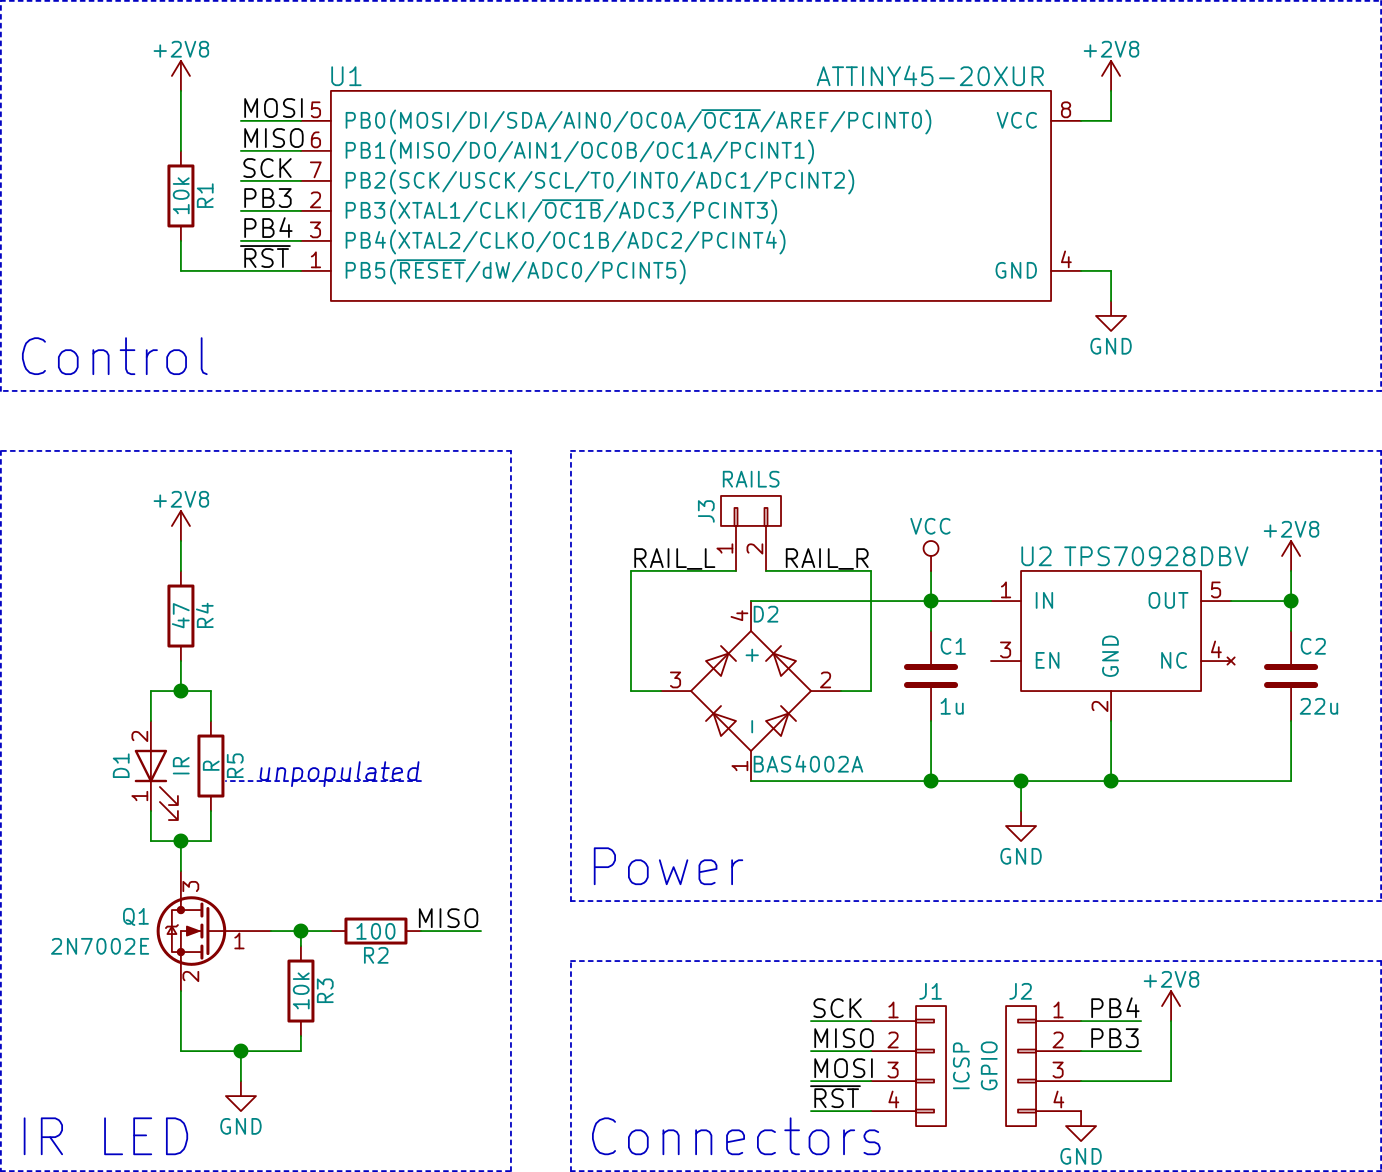
\includegraphics[height=32em]{../electronics/beacon/v1.1/images/beacon-sch-small.png}
\end{center}

\subsection{Locomotive}
\begin{center}
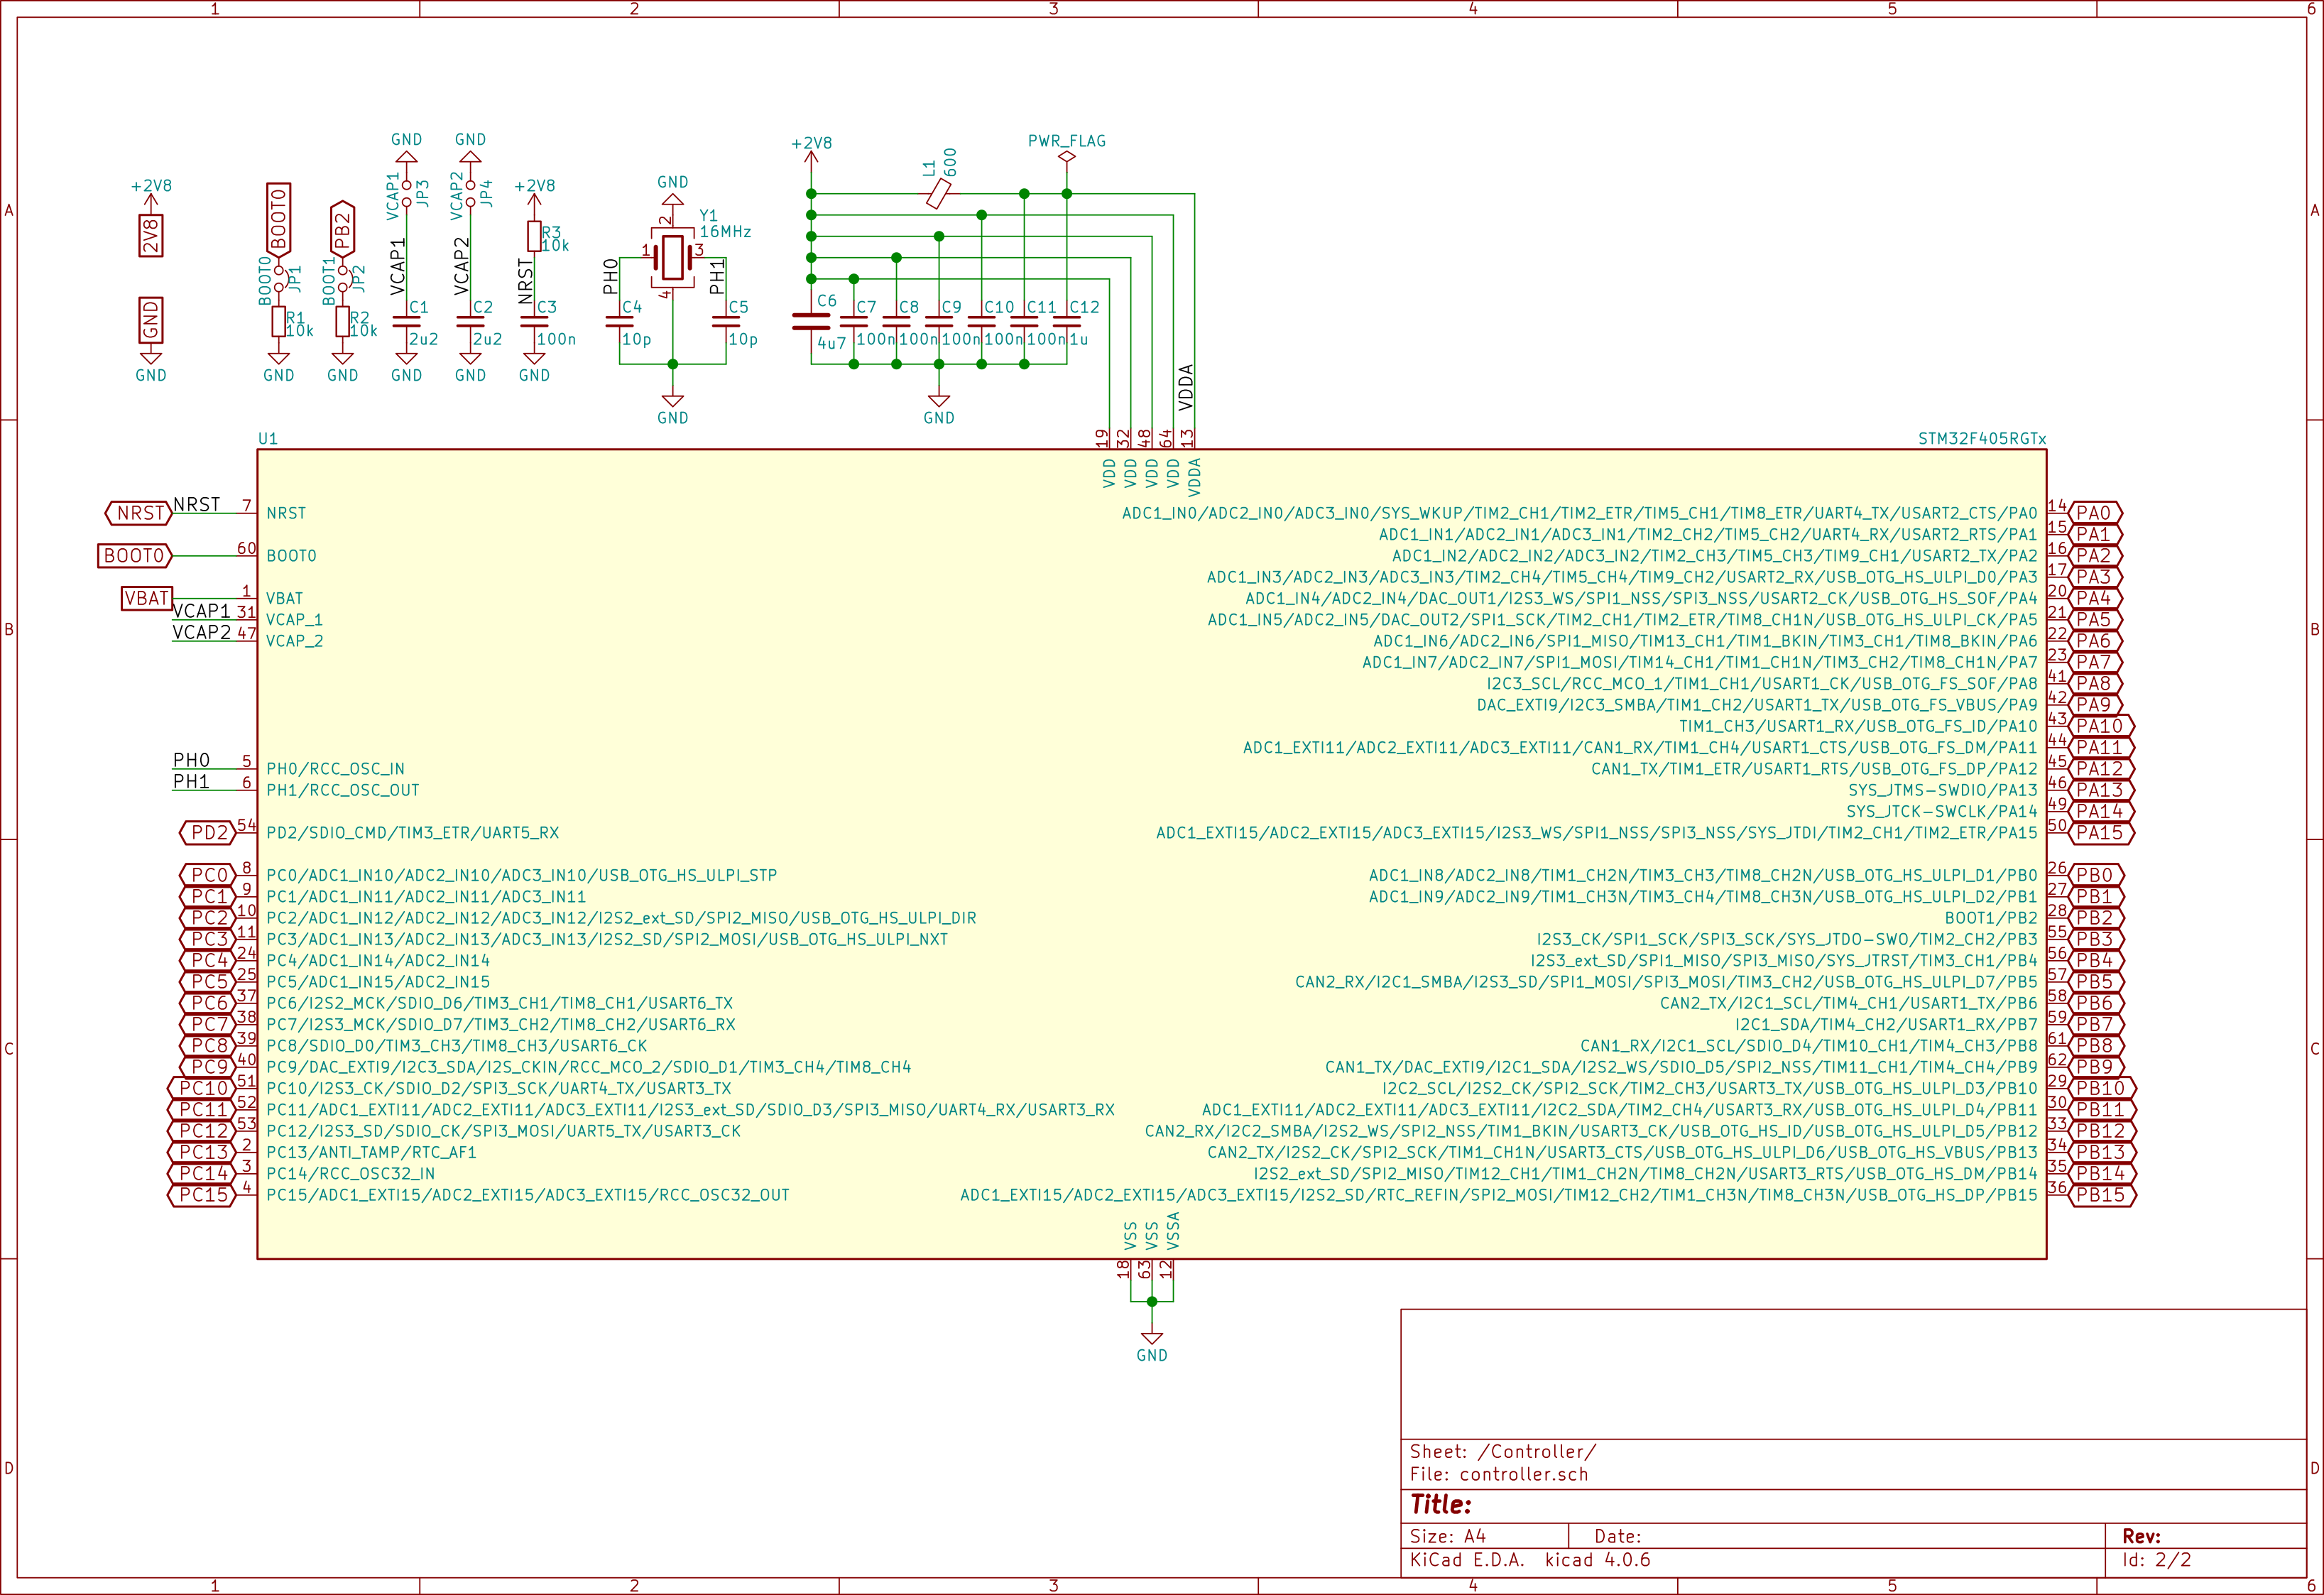
\includegraphics[height=30em]{../electronics/locomotive/images/locomotive-Controller.png}
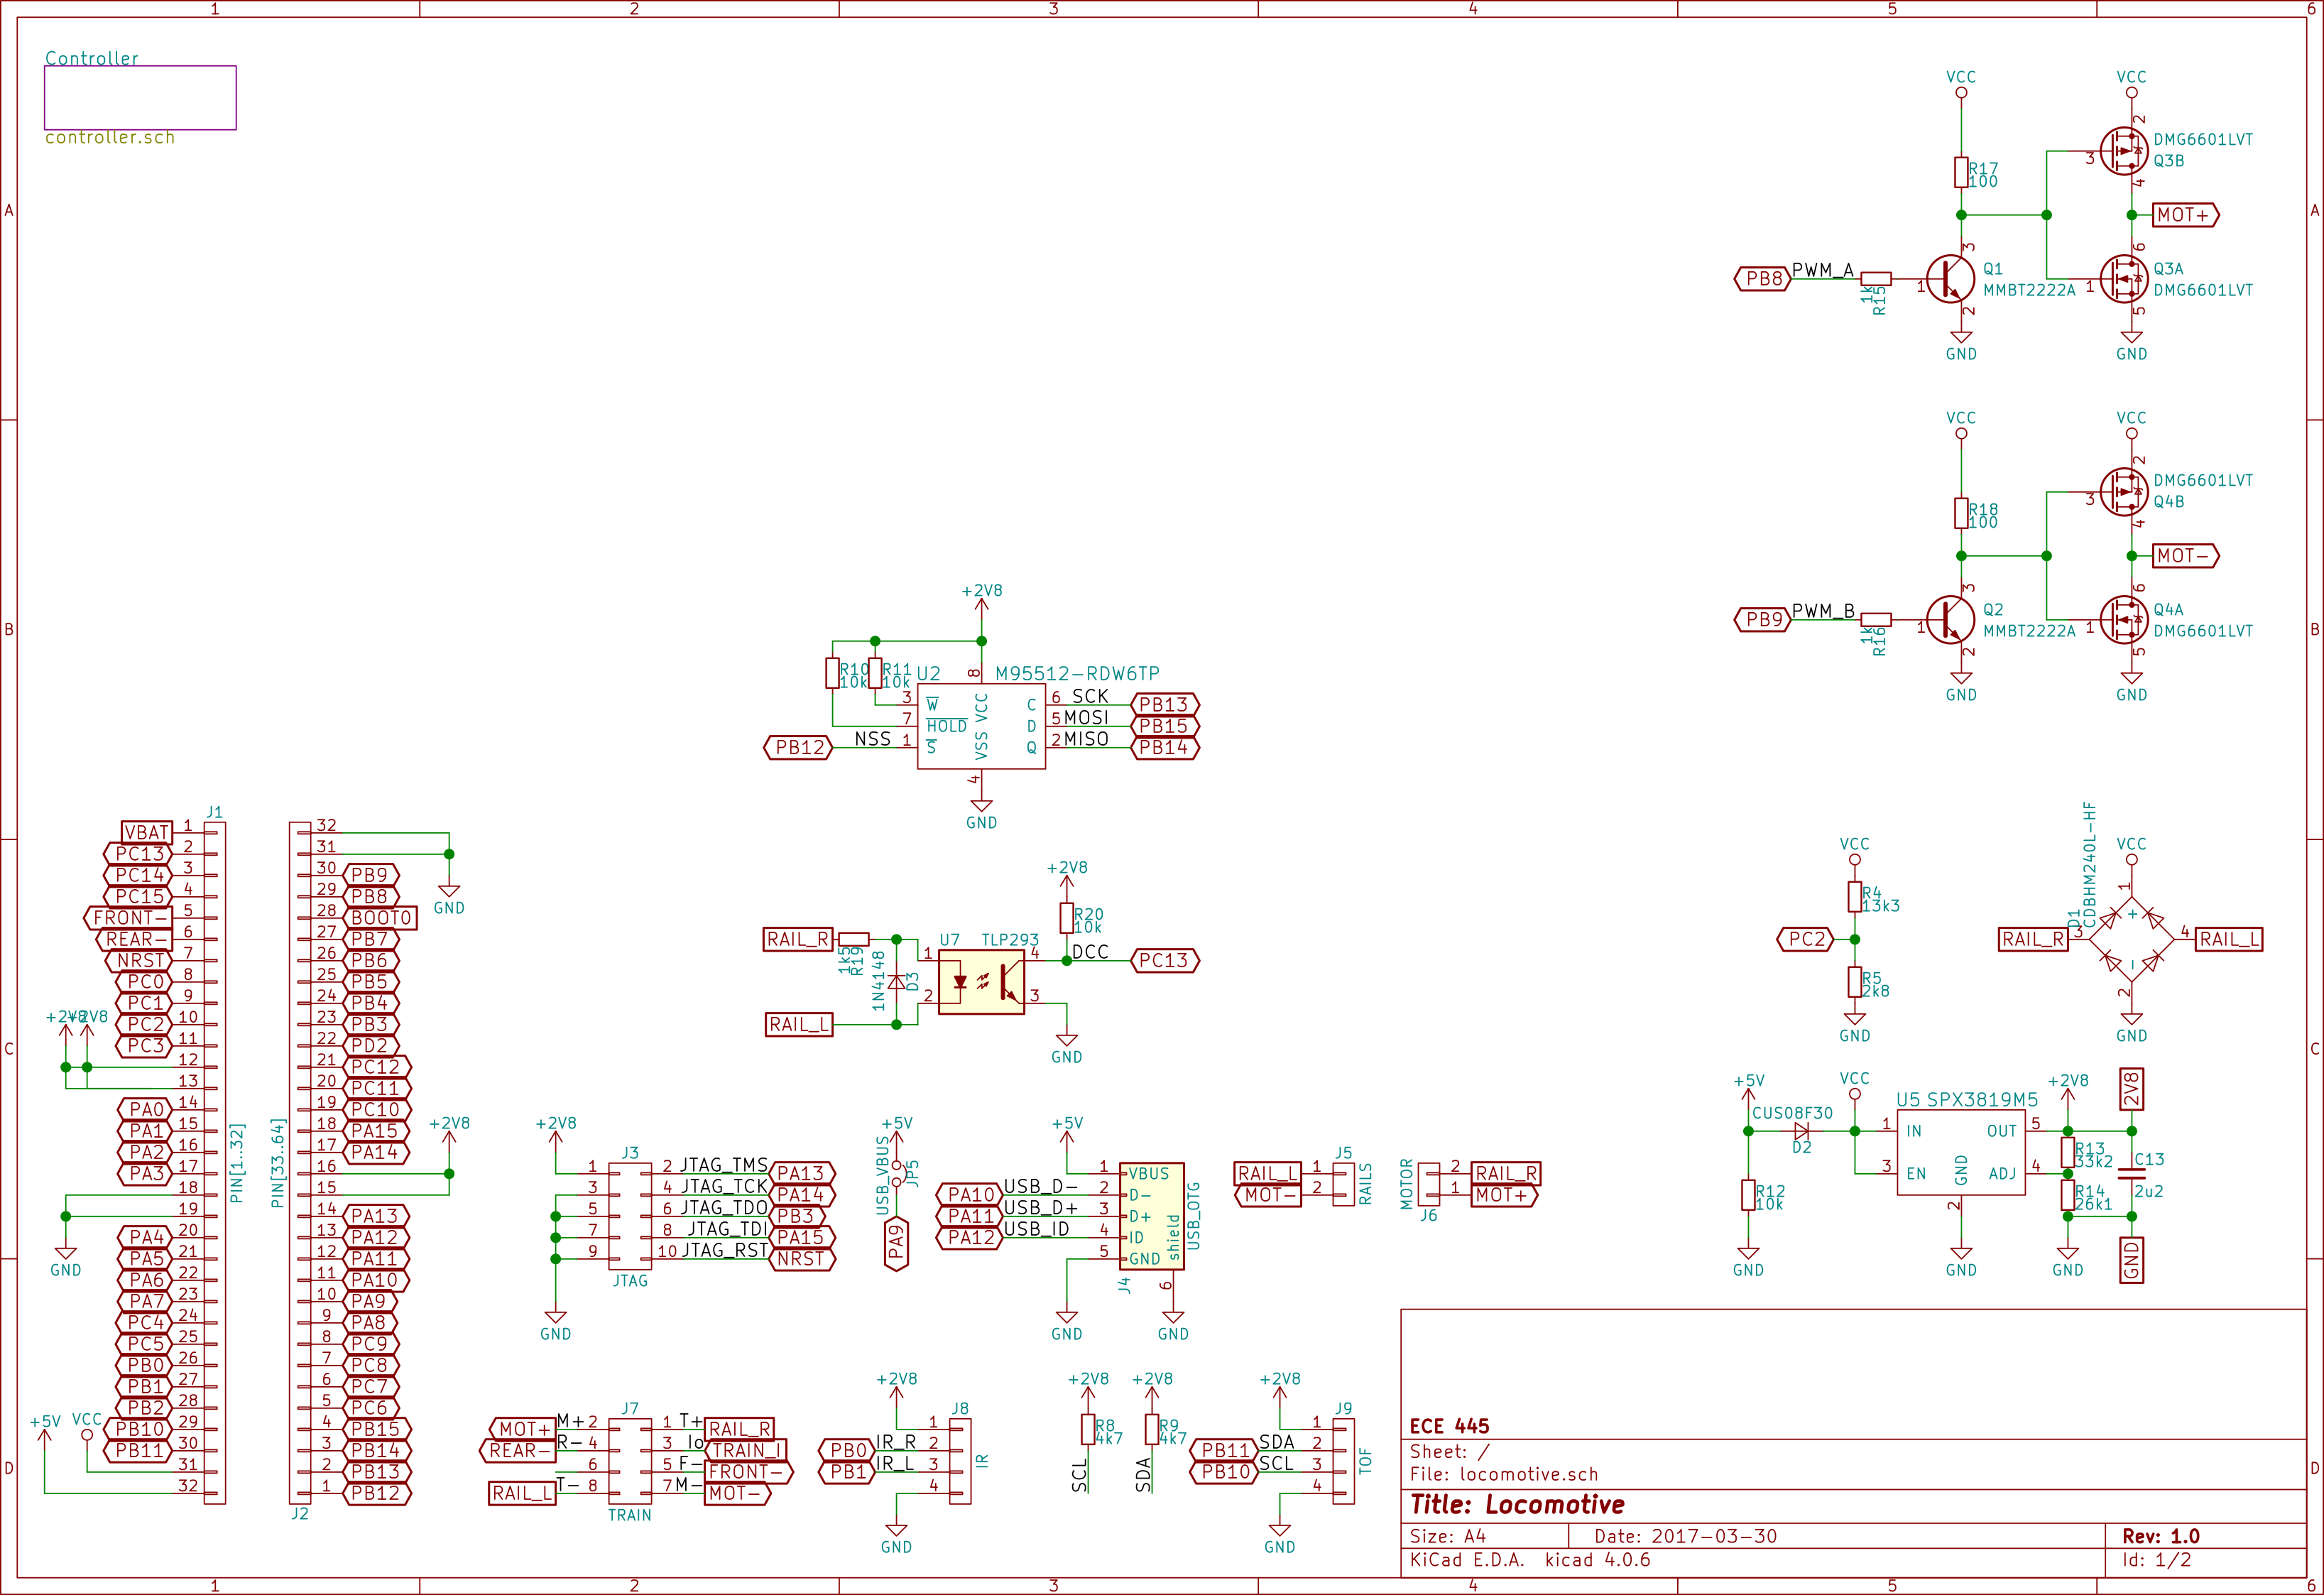
\includegraphics[height=30em]{../electronics/locomotive/images/locomotive-sch.png}
\end{center}

\subsection{Obstacle Detector}
\begin{center}
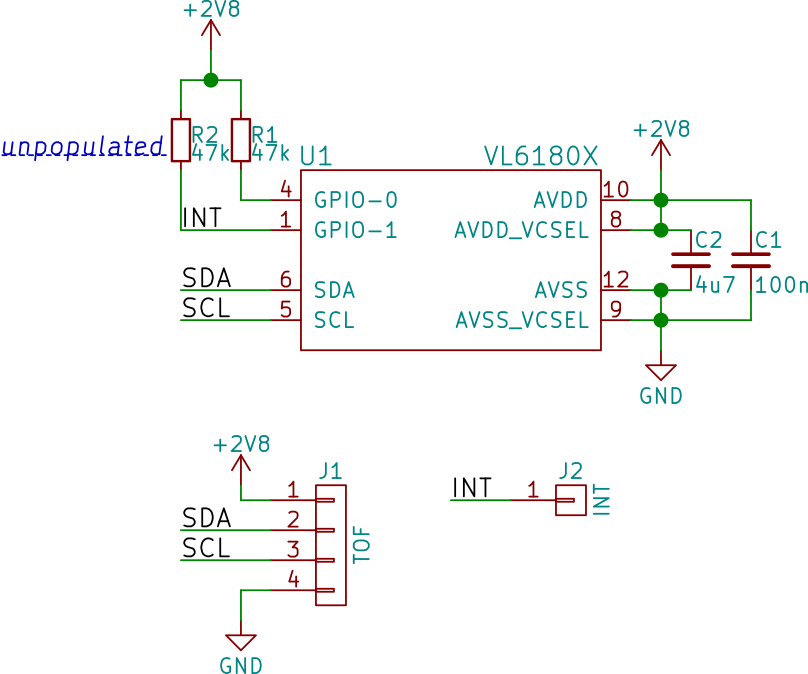
\includegraphics[height=30em]{../electronics/locomotive_tof_sensor/images/locomotive_tof_sensor-sch-small.png}
\end{center}

\subsection{Beacon Reader}
\begin{center}
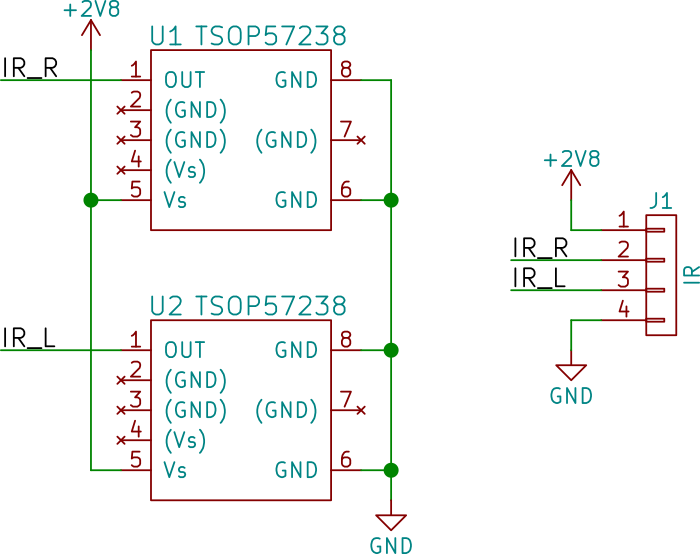
\includegraphics[height=24em]{../electronics/locomotive_ir_receiver/images/locomotive_ir_receiver-sch-small.png}
\end{center}

\clearpage

\section{Pinouts}

\clearpage

\section{Software}

\clearpage

\section{Cost}

\subsection{Beacon BOM}

\subsection{Locomotive BOM}

\subsection{Obstacle Detector BOM}

\subsection{Beacon Reader BOM}

\end{appendix}


\end{spacing}
\end{document}
